\section{Continuous-time continuous-state Markov process}

The mathematical language to study diffusion theory, as with many other field of
science is the language of probability theory. As Jaynes' famous book title
suggested, \textit{probability theory is the logic of science}. It is through
this formal language that we can assess how likely are specific events to
happen. For example, later on we'll see that within the framework of diffusion
theory is possible to ask what is the probability of an allele being fixed in
the population given the evolutionary forces acting on it. But before jumping
into the main topic of this section we need to build up our mathematical
toolkit. In particular we need a way to describe how a quantity of interest -
allele frequency in our case - evolves over time. This is where the language of
stochastic processes becomes very handy to have.

\subsection{Stochastic process}

When describing how a quantity evolves over time with a non-deterministic
trajectory we often use what is commonly known as stochastic processes. For
example imagine we are keeping track of a random variable $X$ that changes over
time. This stochastic variable $X$ could describe things such as count of a
specific chemical species, average price of an asset over a period of time,
frequency of a particular allele on a population, etc. To describe how this
variable $X$ changes over time we could in principle list an infinite number of
functions
\begin{equation}
  X(t) = f(X, t).
\end{equation}
This is what we call a stochastic process, i.e. the time evolution of a random
variable $X$. What we are doing here is considered notation abuse by the more
scrupulous mathematicians. Usually people prefer to define a random process as
$Y_X(t) \equiv f(X, t)$ to specify that we are studying how a random variable
$X$ evolves over time $t$ without compromising the use of $X$ as the sole random
variable, but I personally find that notation too strict. Most of our efforts in
these notes will go into describing the probability distribution of such
processes $P(x, t)$, i.e. the probability of our particular random process
taking the specific value $X(t) = x(t)$. More on that later.

Let's clarify all these subtle but important notation differences: The random
variable $X$ is a mapping from a random event to the real line; in other words,
for a particular quantity that we want to describe we assign a number to
represent the event that happened. A useful example is to think about it as
getting to observe a specific face once we roll a die, and assigning a number
from 1 to 6 to represent the face we observed. The stochastic process $X(t)$
describes the values that our random variable $X$ can take over time. Following
up with the die example this could be rolling a die every so often and keeping
track of the numbers that we obtain. This process $X(t)$ represents the
\textbf{ensemble} of possible realizations $x(t)$. In other words, as shown
schematically in \fref{fig01_00001} $X(t)$ describes all possible values that
the quantity $X$ can take over time, and $x(t)$ describes a specific trajectory
that happened to occur for a specific realization of the process.

\begin{figure}[h!]
	\centering 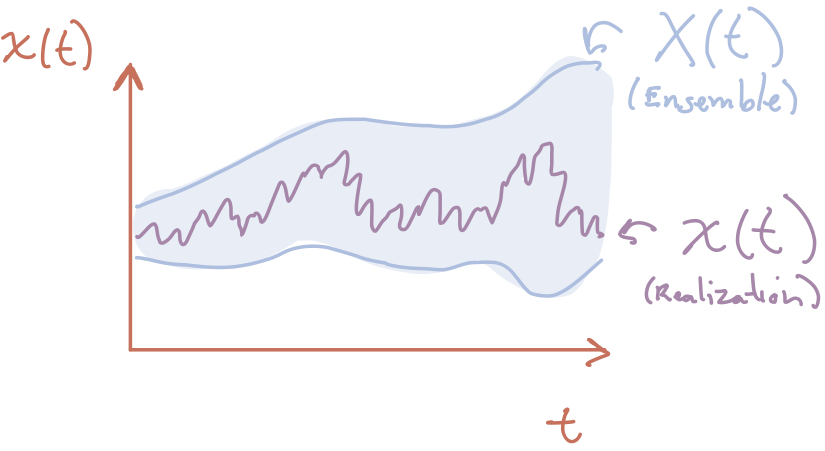
\includegraphics[width=0.5\textwidth]
  {./fig/chapter_prob/01_00001.jpeg}
	\caption{\textbf{Schematic description of a stochastic process}. The shaded
	region describes the stochastic process $X(t)$, i.e. all the possible values
	that the random variable $X$ can take over time. The particular realization
	$x(t)$ describes a specific trajectory that the random variable $X$ took in
	one particular case.}
  \label{fig01_00001}
\end{figure}

From the intuition presented in \fref{fig01_00001} we understand that all possible
trajectories that our stochastic process can take are contained in the function
$X(t)$. But some particular paths $x(t)$ are more likely to happen than others.
This is what the language of probability theory allows us to compute! In
principle we are interested in writing how likely it is for our process to take
a specific value $x(t)$. This is described by the probability function $P(x, t)$
which will be at the center of our endeavors for these notes. Once we define our
stochastic process we might want to compute a moment of the distribution. Recall
that for a continuous random variable $X$ with probability distribution
$P_X(x)$, a moment is defined as
\begin{equation}
  \ee{X^m} \equiv \int dx \; x^m P_X(x),
\end{equation}
where the integral is taken over all the values that $X$ can take. Notice that
our notation for the distribution $P_X(x)$ highlights that we are only
considering the values that $X$ can take, no time involved so far. For our case
in which the random variable can change over time what we have to do is settle
for a specific time point $t^*$ and compute the average at that time point
\begin{equation}
  \ee{X(t^*)^m} \equiv \int dx \; x^m P(x, t^*).
  \label{eq_process_moment}
\end{equation}
Notice that this is still not making a statement about the time evolution of our
variable $X$, but rather committing to a specific time point $t^*$ and then
computing the $m\tth$ moment at that time point. An intuitive way to think about
this is to take a frequentist approach for probability. We imagine that we get
to observe many many individual trajectories $\{x_1(t), \ldots x_n(t)\}$, as
schematically shown in \fref{fig01_00002} then what \eref{eq_process_moment} is
doing is computing the moment at a specific time point $t^*$ highlighted also
in \fref{fig01_00002}.

\begin{figure}[h!]
	\centering 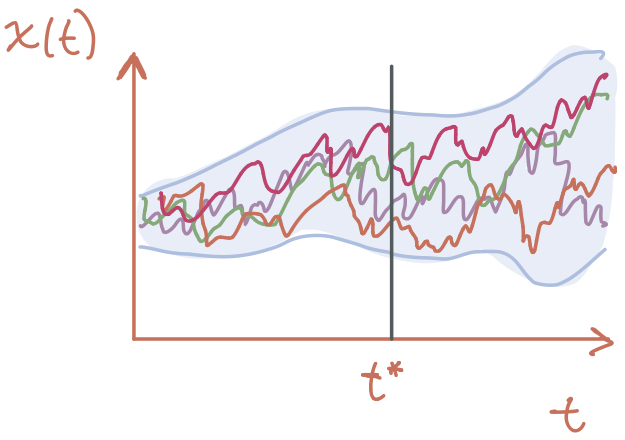
\includegraphics[width=0.5\textwidth]
  {./fig/chapter_prob/01_00002.jpeg}
	\caption{\textbf{Computing a moment of a distribution $\ee{X(t)}$}. Multiple
  realizations of the stochastic process $\{x_1(t), \ldots x_n(t)\}$ are
  highlighted. In the limit where we have many many of these trajectories we
  can then compute a moment of the distribution $P(x, t^*)$ for a specific time
  point $t^*$. \mrm{need better caption}}
  \label{fig01_00002}
\end{figure}

There is no reason why we have to limit ourselves to a single time point $t^*$.
In particular there are interesting quantities such as the autocorrelation
function $\kappa(t_1, t_2)$ that analyze how two different time points $t_1$
and $t_2$ covary with each other. This quantity is defined as
\begin{equation}
  \kappa(t_1, t_2) = \ee{\left(X(t_1) - \ee{X(t_1)}\right)
                         \left(X(t_2) - \ee{X(t_2)}\right)}.
\end{equation}
\mrm{Not sure if I will need to include this if we don't ge to compute moments
that refer to multiple time points.}

Now that we have partially established the notation and conceptual ideas behind
stochastic processes let's focus on a particular kind known as Markov process.

\subsection{Markov processes}
Of particular interested for our endeavor is the specific mathematical objects
known as Markov processes. The Markovian property - named after Andrey Markov, a
famous Russian mathematician from the XIX century - can be stated as follows:
\begin{tcolorbox}
  A Marvov process is a type of stochastic process for which the transition
  states only depends on the current state.
\end{tcolorbox}
To gain intuition for what this means imagine we are measuring a variable $x$
over time such that we have a bunch of pairs of the form $(x_1, t_1), (x_2,
t_2), (x_3, t_3), \ldots (x_{n+1}, t_{n+1})$. For a Markov process, the
probability of ending at state $x_{n+1}$ at time $t_{n+1}$ given all the
previous visited states is of the form
\begin{equation}
  P(x_{n+1}, t_{n+1} \mid x_1, t_1; x_2, t_2; \ldots; x_n, t_n) =
  P(x_{n+1}, t_{n+1} \mid x_n, t_n).
  \label{eq_chapman_kolmogorov}
\end{equation}
In other words, knowing the entire history of variable $x$ as it evolves over
time does not help us predict the next time step. All we need to know is the
last position. Markov processes are usually called memoryless stochastic process
because of this property that the process doesn't remember the full trajectory
when it ``decides'' where to move in the next step. Assuming a Markovian process
is arguably one of the most widely used assumptions in all of science; from
chemical reactions, to brownian motion of a particle, to our particular case of
interest of allele frequencies changing over time.

In the classic formulation of diffusion theory we are concerned with a
particular type of Markov processes. Diffusion theory works in the limit of
large populations where we can assume that the frequency of a particular allele
rather than being a discrete entity that changes in factors of $1 / N$ where
$N$ is the number of organisms, is a continuous value in the range between 0
and 1. We also assume that we can compute changes in this frequency in
continuous time. That means that both $f$ the frequency of an allele, and $t$
the time are continuous variables. Therefore we are interested in a type of
Markov processes that go by the creative name of continuous-time
continuous-state Markov processes. We will now state a very important equation
for this type of Markovian processes known as the Chapman-Kolmogorov equation.

\subsection{Chapman-Kolmogorov equation}

The Chapman-Kolmogorov equation is an important property of continuous-time
continuous-state Markov processes that we will use for many of our derivations
in the coming sections. The equation is stated as follows: For three time points
$t_1 < t_2 < t_3$ for which we measured a stochastic variable $x$ we have that
\begin{equation}
  P(x_3, t_3 \mid x_1, t_1) = \int dx_2\; P(x_3, t_3 \mid x_2, t_2)
                                          P(x_2, t_2 \mid x_1, t_1),
\end{equation}
where the integral is taken over the domain of values that the random variable
$x$ can take. In other words, to calculate the transition probability between
$x_1$ and $x_3$ with an intermediary step $x_2$, we must add (integrate for
continuous variables) all possible values that $x_2$ can take. This concept is
schematically represented in \fref{fig01_00001}

\begin{figure}[h!]
	\centering 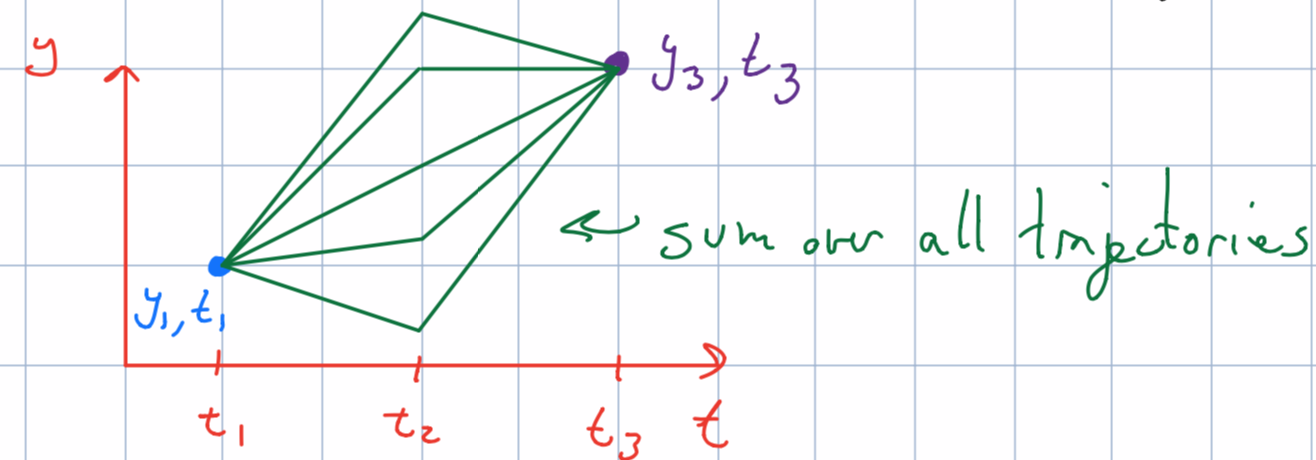
\includegraphics[width=0.5\textwidth]
  {./fig/chapter_prob/01_00003.png}
	\caption{\textbf{Schematic of the Chapman-Kolmogorov equation}. The
  Chapman-Kolmogorov equation is a statement about the transition between two
  points $x_1$ and $x_3$, adding all possible intermediary steps $x_2$.}
  \label{fig01_00003}
\end{figure}

In the coming section we will use the Chapman-Kolmogorov equation to derive the
so-called continuous master equation. This will be the foundation from which we
will get to the main results of diffusion theory. But before jumping into such
matter we need to introduce a specific subtype of Markov processes.

\subsection{Stationary Markov Process}\label{sec_stationary_process}

When thinking about evolution we often summon the concept of a mapping between
genotype (sequence level description) to phenotype (observable characteristic)
to fitness (reproductive success). This concept goes by several names, but in
1932 Sewall Wright attempted to formalize this idea as \textit{adaptive
landscapes}. The phenotype itself can be a function of the genotype and the
environmental state that can itself change over time either deterministically
or stochastically. Therefore the idea of a ``landscape'' is not necessarily the
best description. Some authors have discussed concepts such as \textit{fitness
seascapes} when the environment evolves over time independently of the organism
or \textit{fitness snowscapes} when there is a direct interaction between
organisms modifying the environment, and the environment modifying the
organisms.

For simplicity we usually work with fixed fitness landscapes. This approximation
is valid under certain time-scale regimes. For example, if the environment does
change over time, but it does it on a time-scale much longer than what it takes
for organisms to adapt, then we can pretend for our calculations that the
environment is fixed, simplifying the math enormously. For this particular case
where the mapping all the way from genotype to fitness is not a function of time
is described by a type of stochastic chain known as \textbf{stationary Markov
process}. The formal definition of a stationary Markov process can be stated as
\begin{tcolorbox}
  A stationary Markov process is a memoryless process for which when computing
  the moments of the distribution, these are not affected by a time shift
  $\tau$, i.e.
  \begin{equation}
    \ee{X(t_1 + \tau) X(t_2 + \tau) \cdots X(t_n + \tau)} =
    \ee{X(t_1) X(t_2) \cdots X(t_n)}.
  \end{equation}
\end{tcolorbox}
In other words, for a stationary Markov process what matters are the absolute
time differences $|t_2 - t_1|$ rather than the absolute time points. This
implies that the probability of our random variable having a particular value
$x$ is governed by a probability distribution $P_X(x)$ with no time dependence.
Notice the difference between the statements: On the one hand if we want to know
what is the probability of the random variable transitioning from a value $x$ to
a value $x'$ all we need to know is how much time passed between both
instances of the random process. On the other hand if we are only interested in
knowing what is the probability of the random variable taking a specific value
there is no time dependence for a stationary process since this probability will
not change over time. For the evolution questions we will be addressing here is
easy to see how this implies a fixed adaptive landscape. Since the environment
is fixed the mapping between genotype all the way to fitness will be the same
regardless of the time at which the population acquires a specific allele
frequency.

Now we are ready to derive the master equation that will describe the time
evolution of the probability distribution of allele frequencies.
